\frameT{Outline}{
  \begin{enumerate}
    {\transparent{0.2} \item The languages of PLP-trees and LP-trees}
    \item Learning preference models in case of PLP-trees
    {\transparent{0.2} \item Reasoning with preferences:
      \begin{itemize}
        \item Computing winners and ``strong" candidates when votes are LP-trees
        \item Application in trip planning
      \end{itemize}}
    {\transparent{0.2} \item Future research directions}
  \end{enumerate}
}

%\frameT{The Cars Domain}{
%  \begin{enumerate}
%    \item \tbf{BodyType}(B): \{mvan, sedan, sport, suv\}.
%    \item \tbf{Capacity}(C): \{2, 5, 7m\}.
%    \item \tbf{Color}(O): \{black, blue, gray, red, white\}.
%    \item \tbf{LuggageSize}(L): \{big, med, small\}.
%    \item \tbf{Make}(M): \{bmw, ford, honda, vw\}.
%    \item \tbf{Price}(P): \{low, med, high, vhigh\}.
%    \item \tbf{Safety}(S): \{low, med, high\}.
%  \end{enumerate}
%}

\frameT{Learning PLP-trees}{
	\begin{block}{Consistent Learning (\tsc{ConsLearn})}
		Given an example set $\cE$, decide 
		whether there exists a PLP-tree $T$ (of a particular type) such that $T$ 
		is consistent with $\cE$.
	\end{block}
	\vspace{-0.3cm}

  \begin{figure}[ht]
     \small
    \centering
    \begin{subfigure}[b]{0.95\textwidth}
      \centering
      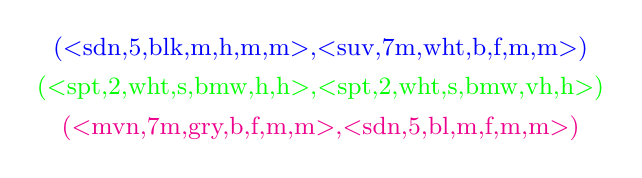
\begin{tikzpicture}[->,>=stealth,node distance=0.5cm,main node/.style={rectangle,font=\small}]
        \node[main node] (1)              {\textcolor{blue}{($<$sdn,5,blk,m,h,m,m$>$,$<$suv,7m,wht,b,f,m,m$>$)}}; 
        \node[main node] (2) [below of=1] {\textcolor{green}{($<$spt,2,wht,s,bmw,h,h$>$,$<$spt,2,wht,s,bmw,vh,h$>$)}};
        \node[main node] (3) [below of=2] {\textcolor{magenta}{($<$mvn,7m,gry,b,f,m,m$>$,$<$sdn,5,bl,m,f,m,m$>$)}};
      \end{tikzpicture}
      %\caption{Examples}
    \end{subfigure}\\ \vspace{0.5cm}
    \begin{subfigure}[b]{0.95\textwidth}
    	\centering
      \begin{tikzpicture}[->,>=stealth',
        level 1/.style={sibling distance=2cm, level distance=33pt},
        level 2/.style={sibling distance=0.7cm, level distance=27pt}
      ]

        \node[main node,inner sep=2pt] (1) {P};
        \node[rectangle,draw,inner sep=2pt] at (1.2,0) {\textcolor{green}{$m \!\!>\!\! h\!\!>\!\! l\!\!>\!\! vh$}};

        \node[main node,inner sep=2pt] (2) [below of=1] {M};
        \node[rectangle,draw,inner sep=2pt] at (1.52,-1) {\textcolor{blue}{$h \!\!>\!\! vw\!\!>\!\! f\!\!>\!\! bmw$}};

        \node[main node,inner sep=2pt] (3) [below of=2] {B};
        \node[rectangle,draw,inner sep=2pt] at (1.8,-2) {\textcolor{magenta}{$mvn\!\! >\!\! suv\!\! >\!\! sdn\!\! >\!\! spt$}};

        \path[every node/.style={font=\sffamily\small}]
          (1) edge (2)
          (2) edge (3);
      \end{tikzpicture}
      \caption*{UIUP tree}
    \end{subfigure}
  \end{figure}
}

\frameT{Learning PLP-trees}{
	\begin{block}{Small Learning (\tsc{SmallLearn})}
		Given an example set $\cE$
		and a positive integer $l$ ($l \leq |\cE|$), decide whether there 
		exists a PLP-tree $T$ (of a particular type) such that $T$ is consistent 
		with $\cE$ and $|T| \leq l$.
	\end{block}
	\vspace{-0.3cm}

  \begin{figure}[ht]
     \small
    \centering
    \begin{subfigure}[b]{0.95\textwidth}
      \centering
      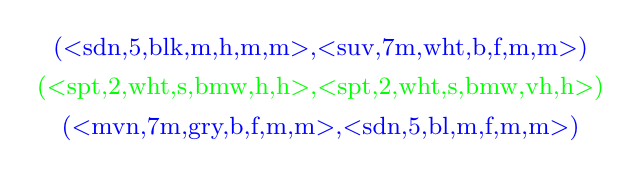
\begin{tikzpicture}[->,>=stealth,node distance=0.5cm,main node/.style={rectangle,font=\small}]
        \node[main node] (1)              {\textcolor{blue}{($<$sdn,5,blk,m,h,m,m$>$,$<$suv,7m,wht,b,f,m,m$>$)}}; 
        \node[main node] (2) [below of=1] {\textcolor{green}{($<$spt,2,wht,s,bmw,h,h$>$,$<$spt,2,wht,s,bmw,vh,h$>$)}};
        \node[main node] (3) [below of=2] {\textcolor{blue}{($<$mvn,7m,gry,b,f,m,m$>$,$<$sdn,5,bl,m,f,m,m$>$)}};
      \end{tikzpicture}
      %\caption{Examples}
    \end{subfigure}\\ \vspace{0.5cm}
    \begin{subfigure}[b]{0.95\textwidth}
    	\centering
      \begin{tikzpicture}[->,>=stealth',
        level 1/.style={sibling distance=2cm, level distance=33pt},
        level 2/.style={sibling distance=0.7cm, level distance=27pt}
      ]

        \node[main node,inner sep=2pt] (1) {B};
        \node[rectangle,draw,inner sep=2pt] at (1.8,0) {\textcolor{blue}{$mvn\!\! >\!\! sdn\!\! >\!\! suv\!\! >\!\! spt$}};

        \node[main node,inner sep=2pt] (2) [below of=1] {P};
        \node[rectangle,draw,inner sep=2pt] at (1.2,-1) {\textcolor{green}{$m \!\!>\!\! h\!\!>\!\! l\!\!>\!\! vh$}};

        \path[every node/.style={font=\sffamily\small}]
          (1) edge (2);
      \end{tikzpicture}
      \caption*{UIUP tree}
    \end{subfigure}
  \end{figure}
}

\frameT{Learning PLP-trees}{
	\begin{block}{Maixmal Learning (\tsc{MaxLearn})}
		Given an example set $\cE$ and a 
		positive integer $k$ ($k \leq m$), decide whether there exists a PLP-tree 
		$T$ (of a particular type) such that $T$ satisfies at least $k$ examples 
		in $\cE$.
	\end{block}
	\vspace{-0.3cm}

  \begin{figure}[ht]
     \small
    \centering
    \begin{subfigure}[b]{0.95\textwidth}
      \centering
      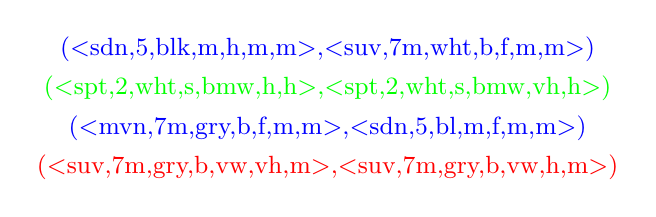
\begin{tikzpicture}[->,>=stealth,node distance=0.5cm,main node/.style={rectangle,font=\small}]
        \node[main node] (1)              {\textcolor{blue}{($<$sdn,5,blk,m,h,m,m$>$,$<$suv,7m,wht,b,f,m,m$>$)}}; 
        \node[main node] (2) [below of=1] {\textcolor{green}{($<$spt,2,wht,s,bmw,h,h$>$,$<$spt,2,wht,s,bmw,vh,h$>$)}};
        \node[main node] (3) [below of=2] {\textcolor{blue}{($<$mvn,7m,gry,b,f,m,m$>$,$<$sdn,5,bl,m,f,m,m$>$)}};
        \node[main node] (4) [below of=3] {\textcolor{red}{($<$suv,7m,gry,b,vw,vh,m$>$,$<$suv,7m,gry,b,vw,h,m$>$)}};
      \end{tikzpicture}
      %\caption{Examples}
    \end{subfigure}\\ \vspace{0.5cm}
    \begin{subfigure}[b]{0.95\textwidth}
    	\centering
      \begin{tikzpicture}[->,>=stealth',
        level 1/.style={sibling distance=2cm, level distance=33pt},
        level 2/.style={sibling distance=0.7cm, level distance=27pt}
      ]

        \node[main node,inner sep=2pt] (1) {B};
        \node[rectangle,draw,inner sep=2pt] at (1.8,0) {\textcolor{blue}{$mvn\!\! >\!\! sdn\!\! >\!\! suv\!\! >\!\! spt$}};

        \node[main node,inner sep=2pt] (2) [below of=1] {P};
        \node[rectangle,draw,inner sep=2pt] at (1.2,-1) {\textcolor{green}{$m \!\!>\!\! h\!\!>\!\! l\!\!>\!\! vh$}};

        \path[every node/.style={font=\sffamily\small}]
          (1) edge (2);
      \end{tikzpicture}
      \caption*{UIUP tree}
    \end{subfigure}
  \end{figure}
}

\frameT{Learning PLP-trees}{
	\begin{block}{Consistent Learning (\tsc{ConsLearn})}
		Given an example set $\cE$, decide 
		whether there exists a PLP-tree $T$ (of a particular type) such that $T$ 
		is consistent with $\cE$.
	\end{block}
	\vspace{-0.3cm}

  \begin{figure}[ht]
     \small
    \centering
    \begin{subfigure}[b]{0.95\textwidth}
      \centering
      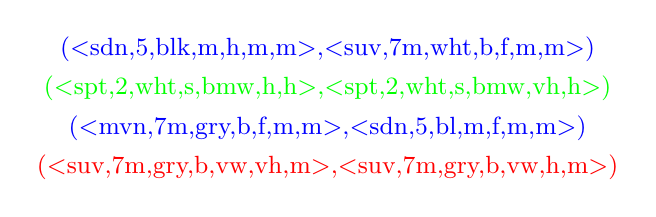
\begin{tikzpicture}[->,>=stealth,node distance=0.5cm,main node/.style={rectangle,font=\small}]
        \node[main node] (1)              {\textcolor{blue}{($<$sdn,5,blk,m,h,m,m$>$,$<$suv,7m,wht,b,f,m,m$>$)}}; 
        \node[main node] (2) [below of=1] {\textcolor{green}{($<$spt,2,wht,s,bmw,h,h$>$,$<$spt,2,wht,s,bmw,vh,h$>$)}};
        \node[main node] (3) [below of=2] {\textcolor{blue}{($<$mvn,7m,gry,b,f,m,m$>$,$<$sdn,5,bl,m,f,m,m$>$)}};
        \node[main node] (4) [below of=3] {\textcolor{red}{($<$suv,7m,gry,b,vw,vh,m$>$,$<$suv,7m,gry,b,vw,h,m$>$)}};
      \end{tikzpicture}
      %\caption{Examples}
    \end{subfigure}\\ \vspace{0.5cm}
    \begin{subfigure}[b]{0.95\textwidth}
    	\centering
      \begin{tikzpicture}[->,>=stealth',
        level 1/.style={sibling distance=2cm, level distance=33pt},
        level 2/.style={sibling distance=0.7cm, level distance=27pt}
      ]

        \node[main node,inner sep=2pt] (1) {B};
        \node[rectangle,draw,inner sep=2pt] at (1.8,0) {\textcolor{blue}{$mvn\!\! >\!\! sdn\!\! >\!\! suv\!\! >\!\! spt$}};

        \node[main node,inner sep=2pt] (2) [below of=1] {P};
        \node[rectangle split, rectangle split parts=4, draw,inner sep=2pt,font=\sffamily\small] at (1.6,-1.5)
            {
              \textcolor{green}{$spt\!:m \!\!>\!\! h\!\!>\!\! l\!\!>\!\! vh$}
              \nodepart{second}
              \textcolor{red}{$suv\!:vh \!\!>\!\! h\!\!>\!\! m\!\!>\!\! l$}
              \nodepart{third}
              $mvn\!:\!m \!\!>\!\! h\!\!>\!\! l\!\!>\!\! vh$
              \nodepart{fourth}
              $sdn\!:\!m \!\!>\!\! h\!\!>\!\! l\!\!>\!\! vh$
            };

        \path[every node/.style={font=\sffamily\small}]
          (1) edge (2);
      \end{tikzpicture}
      \caption*{UICP tree}
    \end{subfigure}
  \end{figure}
}

%\frameT{Learning PLP-trees}{
%	\begin{block}{Consistent Learning (\tsc{ConsLearn})}
%		Given an example set $\cE$, decide 
%		whether there exists a PLP-tree $T$ (of a particular type) such that $T$ 
%		is consistent with $\cE$.
%	\end{block}
%
%	\begin{block}{Small Learning (\tsc{SmallLearn})}
%		Given an example set $\cE$
%		and a positive integer $l$ ($l \leq |\cE|$), decide whether there 
%		exists a PLP-tree $T$ (of a particular type) such that $T$ is consistent 
%		with $\cE$ and $|T| \leq l$.
%	\end{block}
%
%	\begin{block}{Maixmal Learning (\tsc{MaxLearn})}
%		Given an example set $\cE$ and a 
%		positive integer $k$ ($k \leq m$), decide whether there exists a PLP-tree 
%		$T$ (of a particular type) such that $T$ satisfies at least $k$ examples 
%		in $\cE$.
%	\end{block}
%}

\frameT{Computational Complexity}{
  \begin{enumerate}
    \item $P$, $\NP$, $\coNP$: We typically believe that $P \subset \NP$ and $P \subset \coNP$.
    %\item $\coNP$: problems whose complements are in $\NP$.
    \item $\deltap{2}$: $P^\NP$, $\sigmap{2}$: $\NP^\NP$, and $\pip{2}$: $\coNP^\NP$.
    \item $C$-complete: hardest decision problems in class $C$.
    %\item A decision problem $L$ is $C$-hard if $L' \leq_p L$ for every $L'$ in class $C$.
    %\item A decision problem $L$ is $C$-complete if $L$ is in class $C$ and $L$ is $C$-hard.
  \end{enumerate}

  \vspace{-0.3cm}

  \begin{figure}[ht!]
    \centering
      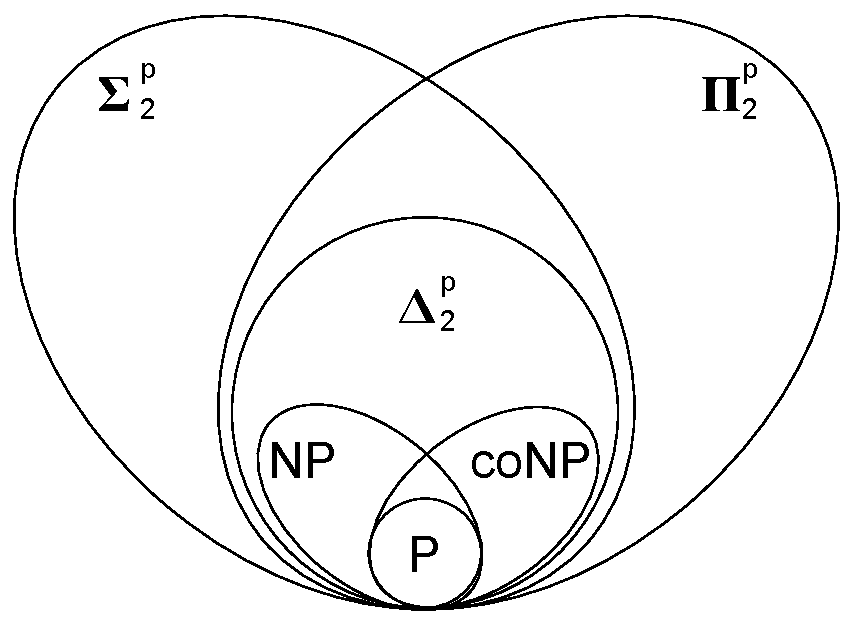
\includegraphics[width=0.5\textwidth]{figs/Preliminary/comp_diagram.pdf}
    \caption{Computational complexity diagram}
  \end{figure}
}

\frameT{Complexity Results on PLP-trees} {
  \begin{figure}[!ht]
    \centering
    \begin{subfigure}[b]{0.45\textwidth}
      \centering
      \begin{tabular}[0.45\textwidth]{ | c | c | c | }
        \hline
           & UP & CP \\
        \hline
        UI & P & P\\
        \hline
        CI & NPC\footnotemark & P  \\
        \hline
      \end{tabular}
      \caption{\tsc{ConsLearn}}
    \end{subfigure}
      \footnotetext{\scriptsize Booth et al., \tit{Learning Conditionally Lexicographic
            Preference Relations}, 2010.}
    \begin{subfigure}[b]{0.45\textwidth}
      \centering
      \begin{tabular}[0.45\textwidth]{ | c | c | c | }
        \hline
           & UP & CP \\
        \hline
        UI & NPC & NPC \\
        \hline
        CI & NPC & NPC \\
        \hline
      \end{tabular}
      \caption{\tsc{SmallLearn}}
    \end{subfigure} \\
    \begin{subfigure}[b]{0.45\textwidth}
      \centering
      \begin{tabular}[0.45\textwidth]{ | c | c | c | }
        \hline
           & UP & CP \\
        \hline
        UI & NPC\footnotemark & NPC \\
        \hline
        CI & NPC & NPC \\
        \hline
      \end{tabular}
      \caption{\tsc{MaxLearn}}
    \end{subfigure}
    \caption{Complexity results for learning PLP-trees}
  \end{figure}
  \footnotetext{\scriptsize Schmitt and Martignon, \tit{On the Complexity of
            Learning Lexicographic Strategies}, 2006.}
}

\frameT{Experimentation}{
  \begin{figure}[ht!]
    \centering
      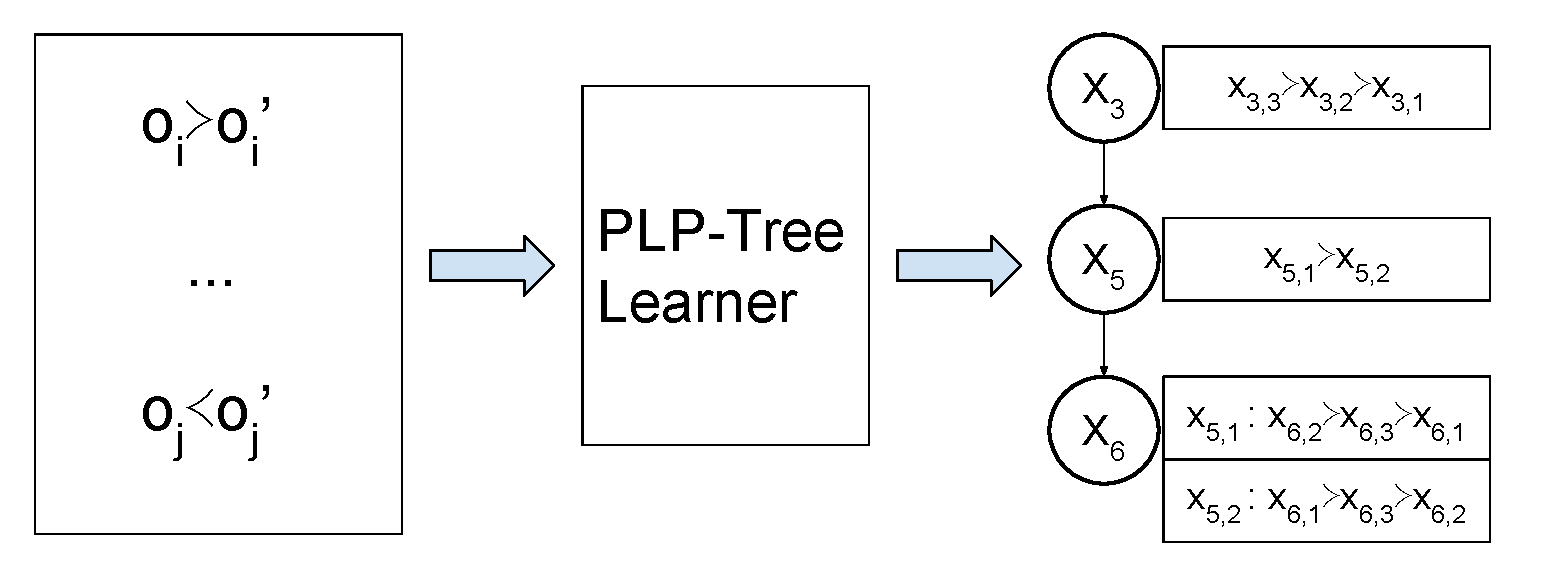
\includegraphics[width=0.9\textwidth]{figs/PrefLearnResults/LearningPLPT.pdf}
    \caption{PLP-tree learning system}
  \end{figure}

}

\frameT{Datasets}{
	\begin{figure}
		\centering
		\begin{tabular}{ |c||c|c|c|c| } 
			\hline
			Dataset          & \#Attributes & \#Objects & \#Examples \\
			\hline \hline
			BreastCancerWisconsin   & 9 & 270 & 9,009 \\ 
			\hline
			CarEvaluation           & 6 & 1,728 & 682,721 \\ 
			\hline
			CreditApproval          & 10 & 520 & 66,079 \\
			\hline
			GermanCredit            & 10 & 914 & 172,368  \\
			\hline
			Ionosphere              & 10 & 118 & 3,472 \\
			\hline
			MammographicMass        & 5 & 62 & 792 \\
			\hline
			Mushroom                & 10 & 184 & 8,448 \\
			\hline
			Nursery                 & 8 & 1,266 & 548,064 \\
			\hline
			SPECTHeart              & 10 & 115 & 3,196 \\
			\hline
			TicTacToe               & 9 & 958 & 207,832 \\
			\hline
			Vehicle                 & 10 & 455 & 76,713 \\
			\hline
			Wine                    & 10 & 177 & 10,322 \\
			\hline
		\end{tabular}
		\caption{Preference Learning Library\footnotemark}
	\end{figure}

	\footnotetext{\tiny \url{http://www.cs.uky.edu/~liu/preflearnlib.php}}
}

\frameT{PLP-Trees To Learn}{
  \begin{figure}[ht!]
    \centering
      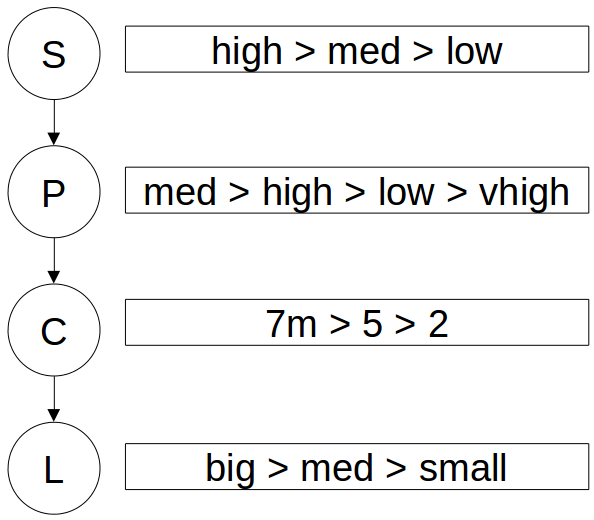
\includegraphics[width=0.4\textwidth]{figs/Cars/uiuptree.png}
    \caption{Unconditional Importance \& Unconditional Preference (UIUP)}
  \end{figure}
}

\frameT{PLP-Trees To Learn}{
  \begin{figure}[ht!]
    \centering
      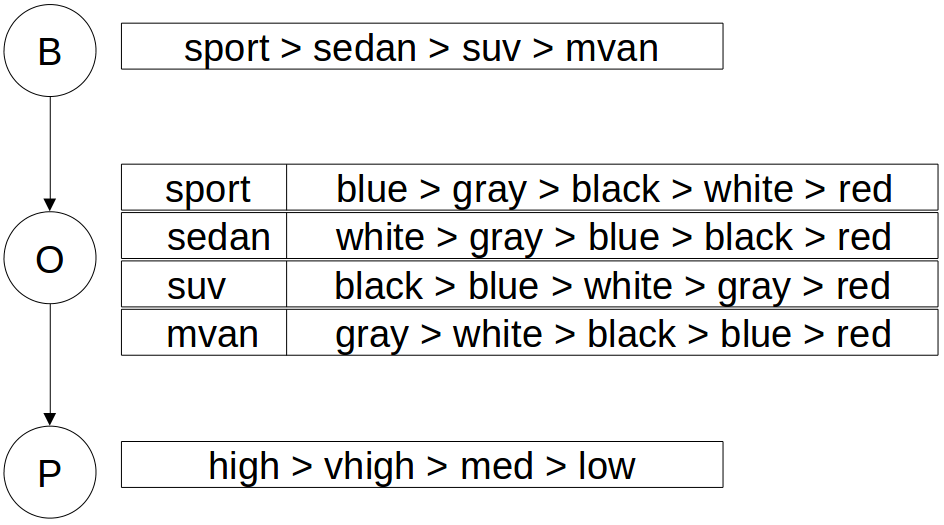
\includegraphics[width=0.65\textwidth]{figs/Cars/uicptree.png}
    \caption{UICP with at most 1 parent (UICP-1)}
  \end{figure}
}

\frameT{PLP-Trees To Learn}{
  \begin{figure}[ht!]
    \centering
      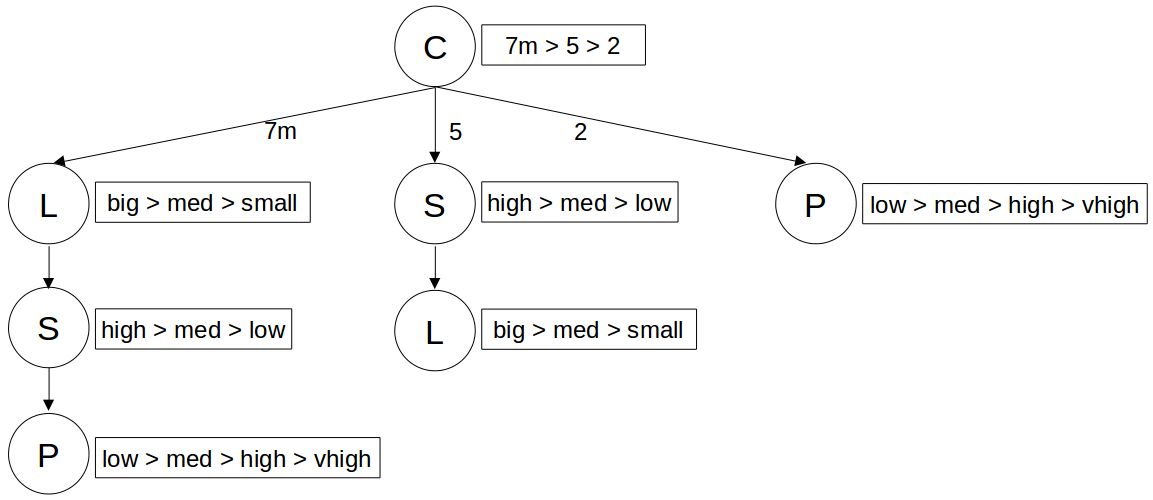
\includegraphics[width=0.9\textwidth]{figs/Cars/ciuptree.png}
    \caption{CIUP with 1 split at the root (CIUP-1)}
  \end{figure}
}

\frameT{PLP-Trees To Learn}{
  \begin{figure}[ht!]
    \centering
      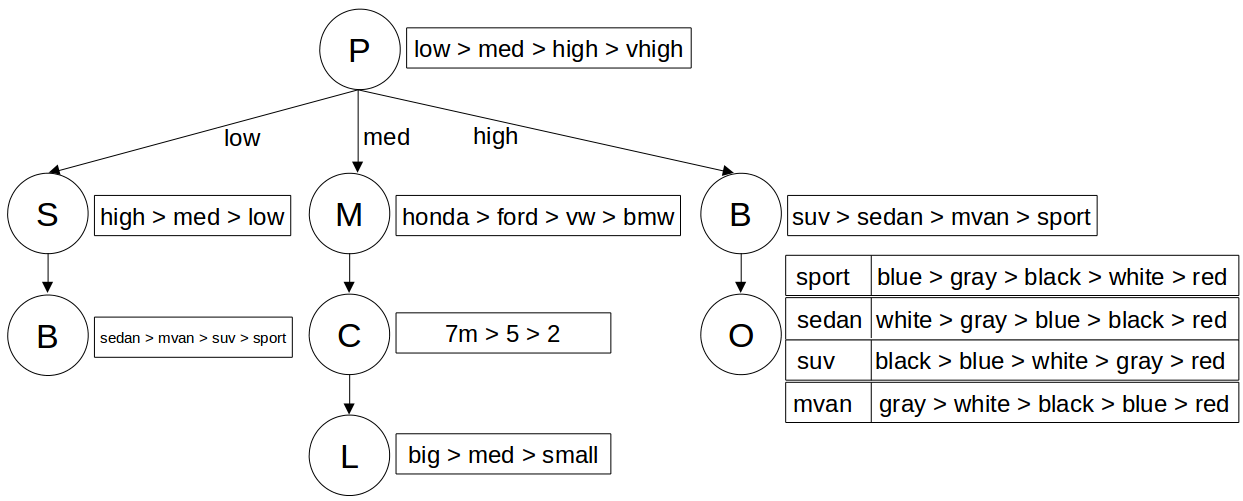
\includegraphics[width=0.9\textwidth]{figs/Cars/cicptree.png}
    \caption{Simple CICP (SCICP)}
  \end{figure}
}

\frameT{Experimental Results: CarEvaluation\footnote{
\tiny \url{http://www.cs.uky.edu/~liu/preflearnlib.php}}
}
{
	\begin{center}
		\#attributes:6, \#objects:1728, \#examples:682721
	\end{center}

  \begin{figure}
    \centering
    \begin{subfigure}[b]{0.48\textwidth}
      \centering
      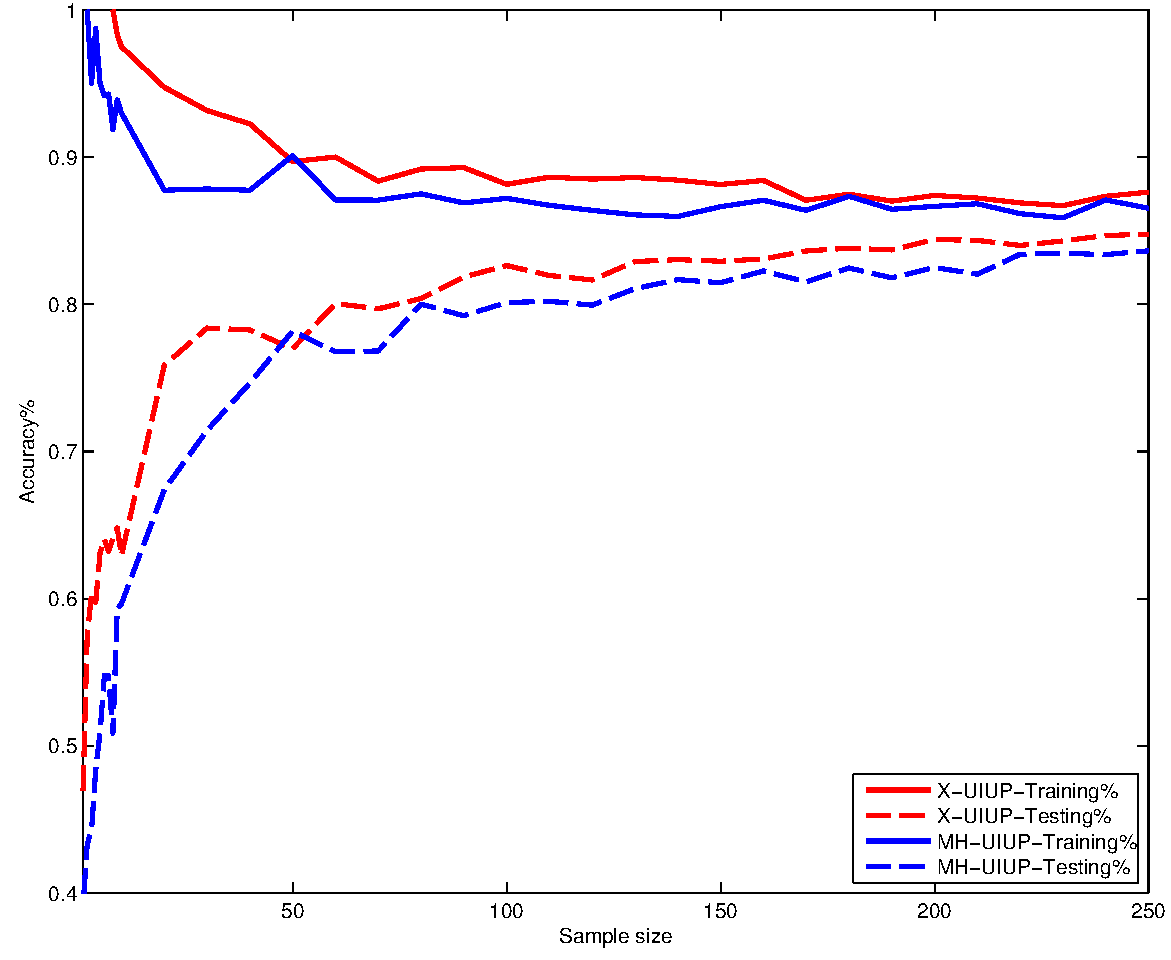
\includegraphics[width=0.95\textwidth]{figs/PrefLearnResults/MatLabOutput/CarEvaluation_Trees_X_MH.pdf}
      \caption{Compare exact \& greedy heuristic}
    \end{subfigure}
    \begin{subfigure}[b]{0.48\textwidth}
      \centering
      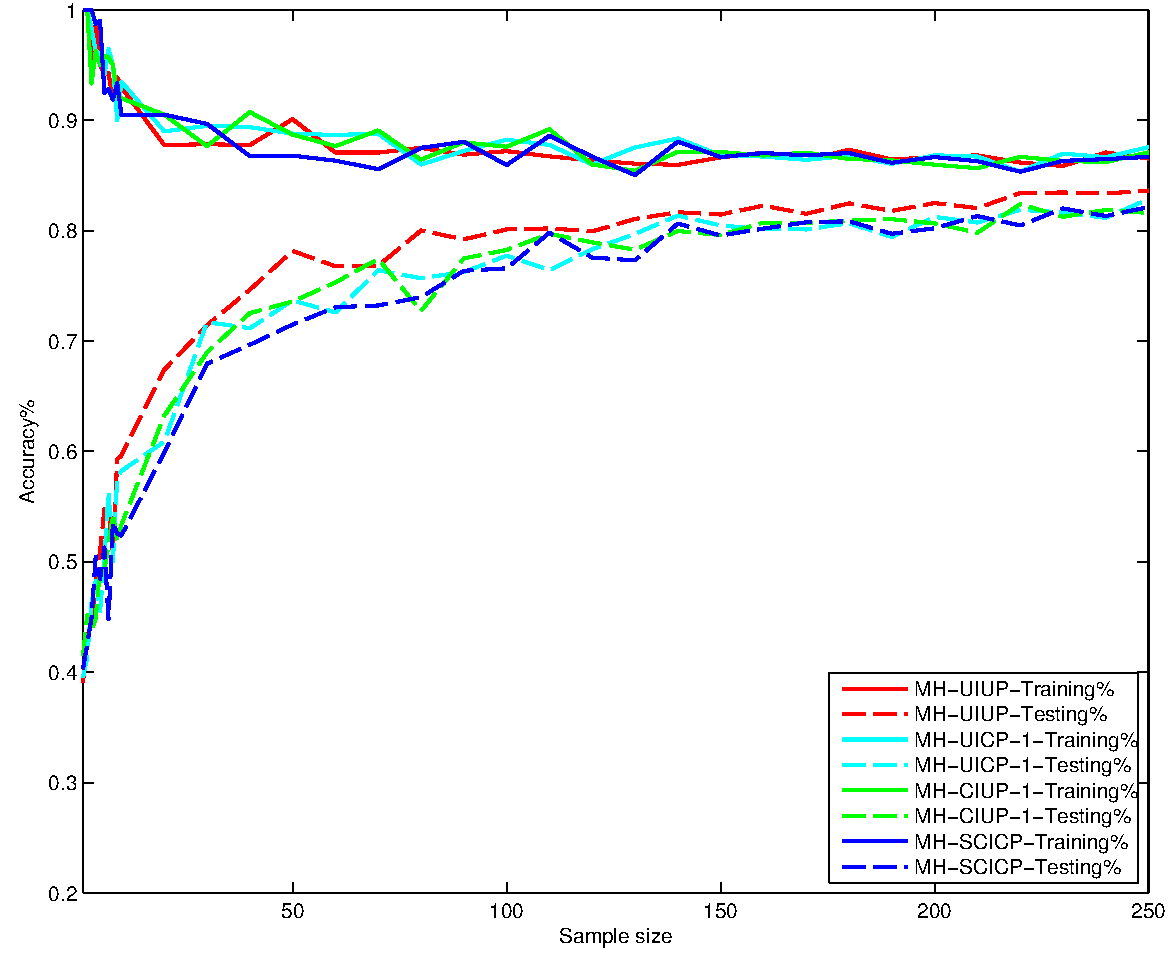
\includegraphics[width=0.95\textwidth]{figs/PrefLearnResults/MatLabOutput/CarEvaluation_Trees_MH.pdf}
      \caption{Greedy heuristic}
    \end{subfigure}

    \caption{Learning curves solving \tsc{MaxLearn}}
  \end{figure}
}

\frameT{Experimental Results: Wine\footnote{
\tiny \url{http://www.cs.uky.edu/~liu/preflearnlib.php}}
}
{
	\begin{center}
		\#attributes:10, \#objects:177, \#examples:10322
	\end{center}

  \begin{figure}
    \centering
    \begin{subfigure}[b]{0.48\textwidth}
      \centering
      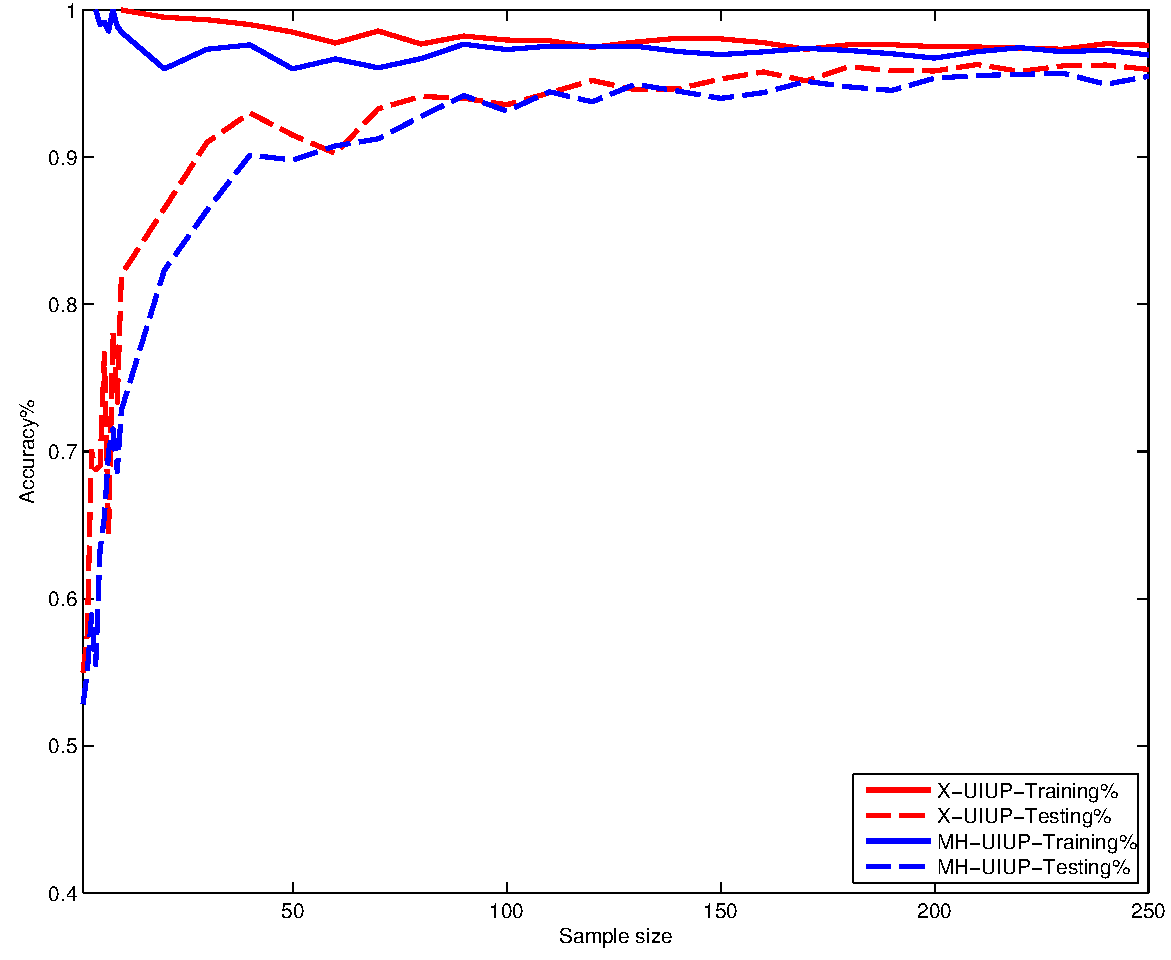
\includegraphics[width=0.95\textwidth]{figs/PrefLearnResults/MatLabOutput/Wine_Trees_X_MH.pdf}
      \caption{Compare exact \& greedy heuristic}
    \end{subfigure}
    \begin{subfigure}[b]{0.48\textwidth}
      \centering
      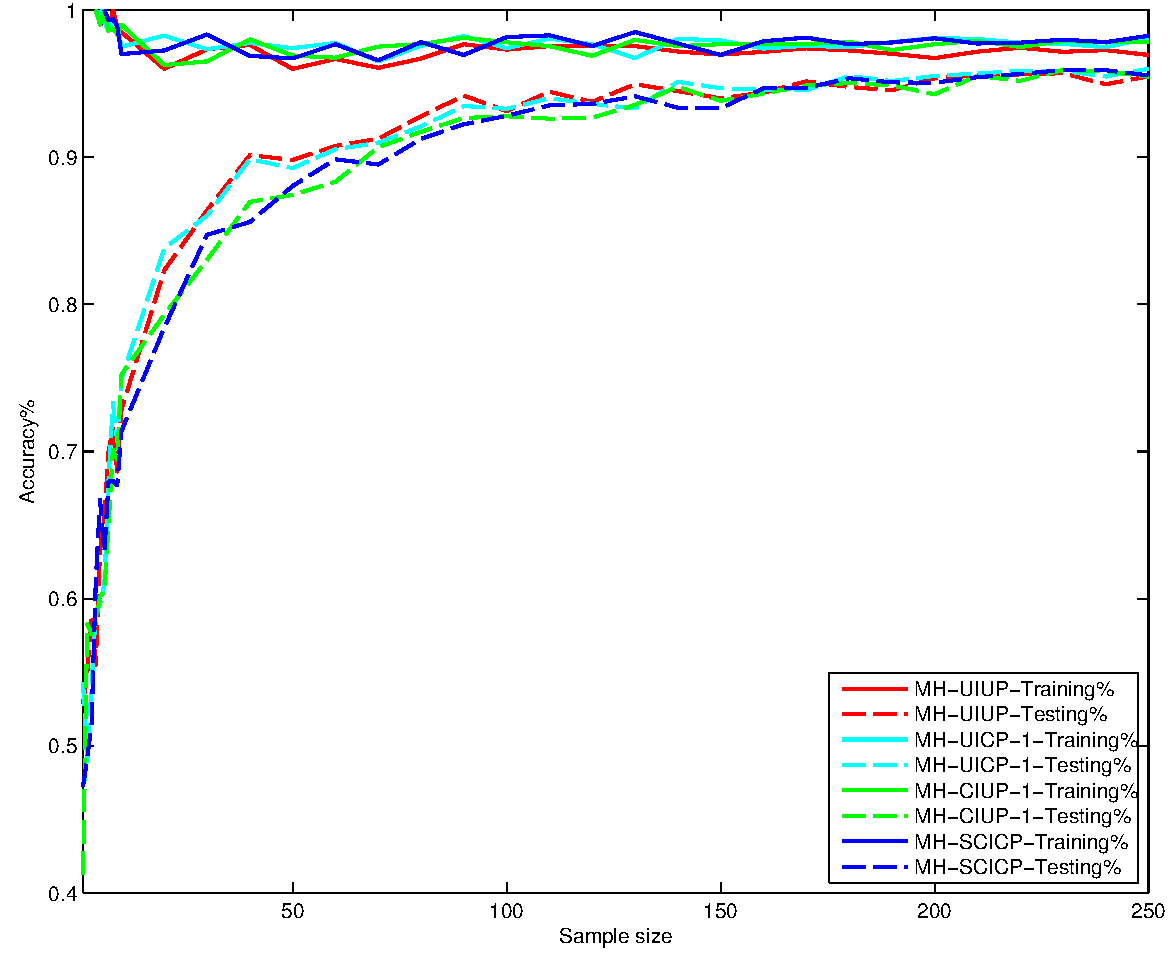
\includegraphics[width=0.95\textwidth]{figs/PrefLearnResults/MatLabOutput/Wine_Trees_MH.pdf}
      \caption{Greedy heuristic}
    \end{subfigure}

    \caption{Learning curves solving \tsc{MaxLearn}}
  \end{figure}
}

%\frameT{Preference Forests (P-Forests)}{
%	\begin{enumerate}
%		\item A \tit{preference forest} $F$ is a collection of PLP-trees
%					$F = \{T_1,\ldots,T_n\}$.
%		\item Denote by $N_F(o_1,o_2)=|\{T \in F:o_1 \succ_T o_2\}|$.
%		\item Given a preference forest $F$, and two outcomes $o_1$ and $o_2$, 
%					we say that $o_1 \succ_F^\Maj o_2$ iff $N_F(o_1,o_2)>N_F(o_2,o_1)$,
%					and that $o_1 \approx_F^\Maj o_2$ iff $N_F(o_1,o_2)=N_F(o_2,o_1)$.
%		\begin{itemize}
%			\item Pro: intuitive, decided in polynomial time.
%			\item Con: Condorcet paradox.
%			\item Other aggregating rules: positional scoring rules, Copeland's method, etc.
%		\end{itemize}
%	\end{enumerate}
%}
%
%\frameT{Experimental Results on P-Forests}{
%  \begin{figure}[ht!]
%    \centering
%      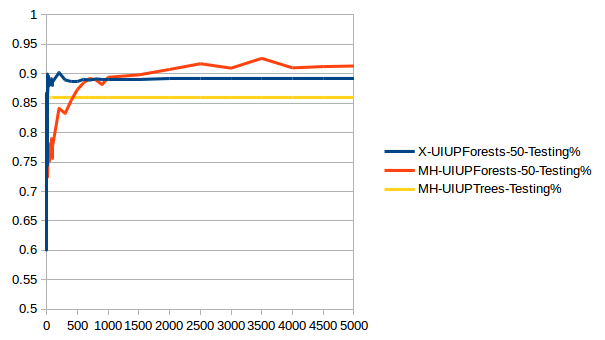
\includegraphics[width=0.7\textwidth]{figs/PrefLearnResults/Forests/X_MH/CarEvaluation.png}
%    \caption{Learning UIUP using ASP and greedy heuristic}
%  \end{figure}
%}
%
%\frameT{Experimental Results on P-Forests}{
%  \begin{figure}[ht!]
%    \centering
%      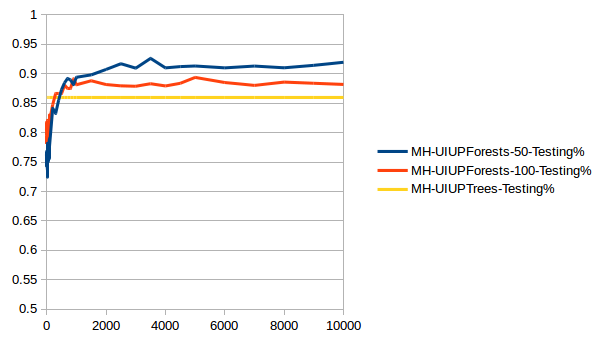
\includegraphics[width=0.7\textwidth]{figs/PrefLearnResults/Forests/MH/CarEvaluation.png}
%    \caption{Learning all four classes using greedy heuristic}
%  \end{figure}
%}
